% gm-11-logarithms.tex

\documentclass[xcolor=dvipsnames]{beamer}

\usepackage{cancel}
\renewcommand{\CancelColor}{\color{red}}
\usepackage{graphicx}
\usepackage{wrapfig}
\usepackage{colortbl}
\usepackage{color}
\usepackage{alltt}
\renewcommand*{\thefootnote}{\fnsymbol{footnote}}
\definecolor{myblue}{rgb}{0.8,0.85,1}

\mode<presentation>
{
  \usetheme{Warsaw}
  \setbeamercovered{transparent}
}
% \usecolortheme[named=OliveGreen]{structure}
\setbeamertemplate{navigation symbols}{} 
\setbeamertemplate{blocks}[rounded][shadow=true] 

% this is for overlaying math symbols, see https://tex.stackexchange.com/questions/12895/overlay-symbol-with-another
\def\qeq{\mathrel{%
    \mathchoice{\QEQ}{\QEQ}{\scriptsize\QEQ}{\tiny\QEQ}%
}}
\def\QEQ{{%
    \setbox0\hbox{$\longrightarrow$}%
    \rlap{\hbox to \wd0{\hss/\hss}}\box0
  }}

\newcounter{expls}
\setcounter{expls}{0}
\newcommand{\beispiel}[1]{\refstepcounter{expls}\textbf{Example \arabic{expls}: #1.}}

\newcounter{exercise}
\setcounter{exercise}{0}
\newcommand{\ubung}[0]{\refstepcounter{exercise}\textbf{Exercise \arabic{exercise}: }}

\newif\ifBCITCourse
\BCITCoursetrue
% \BCITCoursefalse
\newif\ifWhichCourse
\WhichCoursetrue
\WhichCoursefalse
\ifBCITCourse
\ifWhichCourse
\newcommand{\CourseName}{Technical Mathematics for Food Technology}
\newcommand{\CourseNumber}{MATH 1441}
\newcommand{\CourseInst}{BCIT}
\else
\newcommand{\CourseName}{Technical Mathematics for Geomatics}
\newcommand{\CourseNumber}{MATH 1511}
\newcommand{\CourseInst}{BCIT}
\fi
\else
\newcommand{\CourseName}{Philosophy and Literature}
\newcommand{\CourseNumber}{PHIL 375}
\newcommand{\CourseInst}{UBC}
\fi

\title{Logarithms}
\subtitle{{\CourseNumber}, BCIT}

\author{\CourseName}

\date{October 25, 2017}

\begin{document}

\begin{frame}
  \titlepage
\end{frame}

\begin{frame}
  \frametitle{Functions}
Here are a few definitions,
\begin{description}
\item[function] A function assigns a unique element of a set to each
  element of another (not necessarily distinct) set.
\item[domain] The domain is the set of elements to which the function
  assigns a unique element.
\item[codomain] The codomain is the set from which the function picks
  out elements to assign.
\item[range] The range is the subset of the codomain whose elements
  the function assigns to an element in the domain.
\item[injective] A function is injective if it does not assign the
  same element of the codomain to two distinct elements in the domain.
\item[surjective] A function is surjective if there are no elements in
  the codomain which are not assigned to an element in the domain.
\end{description}
\end{frame}

\begin{frame}
  \frametitle{Examples}
What are possible domains and ranges for the following functions? Are
the functions injective or surjective, given a particular domain and
codomain?
\begin{equation}
  \label{eq:rebiejie}
  f(x)=2x+3
\end{equation}
\begin{equation}
  \label{eq:ebaivuim}
  f(x)=x^{2}-1
\end{equation}
\begin{equation}
  \label{eq:ichievae}
  f(x)=\sqrt{x+4}
\end{equation}
\begin{equation}
  \label{eq:ejawache}
  f(x)=\frac{1}{x+7}
\end{equation}
\begin{equation}
  \label{eq:tohjuogi}
  f(x)=10^{2x}
\end{equation}
\end{frame}

\begin{frame}
  \frametitle{Inverse Functions}
If a function $f$ from a domain to a codomain is injective, then there
is a function $f^{-1}$ from the range of $f$ to its domain which has
the following property,
\begin{equation}
  \label{eq:noexiedi}
  f^{-1}(y)=x\mbox{ if and only if }f(x)=y
\end{equation}
We call $f^{-1}$ the \alert{inverse function} of $f$. Let, for
example,
\begin{equation}
  \label{eq:iengaihu}
  f(x)=4x-3
\end{equation}
Replace $f(x)$ by $y$ for the equation $y=4x-3$ and manipulate the
equation to isolate $x$. Then replace $x$ by $f^{-1}(y)$ for the
inverse function
\begin{equation}
  \label{eq:eimoofie}
  f^{-1}(y)=\frac{y+3}{4}
\end{equation}
\end{frame}

\begin{frame}
  \frametitle{Exercises}
  {\ubung} Indicate whether the following functions are injective
  and/or surjective. ($\mathbb{R}^{+}$ is the set of positive real
  numbers.)
\begin{equation}
  \label{eq:oapaedah}
  f_{1}:\mathbb{R}\rightarrow\mathbb{R}\hspace{.5in}f_{1}(x)=\frac{1}{2}x-\frac{7}{3}
\end{equation}
\end{frame}

\begin{frame}
  \frametitle{Exercises}
  {\ubung} Indicate whether the following functions are injective
  and/or surjective. ($\mathbb{R}^{+}$ is the set of positive real
  numbers.)
\begin{equation}
  \label{eq:ariwioga}
  f_{2}:\mathbb{R}\rightarrow\mathbb{R}\hspace{.5in}f_{2}(x)=x^{2}+5
\end{equation}
\end{frame}

\begin{frame}
  \frametitle{Exercises}
  {\ubung} Indicate whether the following functions are injective
  and/or surjective. ($\mathbb{R}^{+}$ is the set of positive real
  numbers.)
\begin{equation}
  \label{eq:aeghahpi}
  f_{3}:\{x\in\mathbb{R}|-4\leq{}x\}\rightarrow\mathbb{R}\hspace{.5in}f_{3}(x)=\sqrt{x+4}
\end{equation}
\end{frame}

\begin{frame}
  \frametitle{Exercises}
  {\ubung} Indicate whether the following functions are injective
  and/or surjective. ($\mathbb{R}^{+}$ is the set of positive real
  numbers.)
\begin{equation}
  \label{eq:lohceuwe}
  f_{4}:\mathbb{R}\setminus\{0\}\rightarrow\mathbb{R}^{+}\hspace{.5in}f_{4}(x)=\left\vert\frac{1}{x}\right\vert
\end{equation}
\end{frame}

\begin{frame}
  \frametitle{Exercises}
  {\ubung} What is the inverse function of the following functions? Specify
the domain of the inverse function.
\begin{equation}
  \label{eq:saleicee}
  g_{1}:\mathbb{R}\rightarrow\mathbb{R}\hspace{.5in}g_{1}(x)=5x-6
\end{equation}
\end{frame}

\begin{frame}
  \frametitle{Exercises}
  {\ubung} What is the inverse function of the following functions? Specify
the domain of the inverse function.
\begin{equation}
  \label{eq:ahnaibio}
  g_{2}:\mathbb{R}\rightarrow\mathbb{R}\hspace{.5in}g_{2}(x)=7^{x+1}
\end{equation}
\end{frame}

\begin{frame}
  \frametitle{Exercises}
  {\ubung} What is the inverse function of the following functions? Specify
the domain of the inverse function.
\begin{equation}
  \label{eq:hegaijou}
  g_{3}:\mathbb{R}^{+}\rightarrow\mathbb{R}\hspace{.5in}g_{3}(x)=\ln{}x
\end{equation}
\end{frame}

\begin{frame}
  \frametitle{Defining Logarithms}
Let $f$ be an exponential function with a base $a>1$,
\begin{equation}
  \label{eq:ohzuiwah}
  f(x)=a^{x}
\end{equation}
Considering the function graph of this exponential function, it is
apparent that $f$ is an injective and surjective function for the
domain $\mathbb{R}$ and the codomain $\mathbb{R}^{+}$.
$\mathbb{R}^{+}$ is the set of all positive real numbers. There is
therefore an inverse function from $\mathbb{R}^{+}$ to the real
numbers, which we shall call $\log_{a}$,
\begin{equation}
  \label{eq:cievucha}
  \log_{a}(y)=x\mbox{ if and only if }a^{x}=y
\end{equation}
\end{frame}

\begin{frame}
  \frametitle{Logarithm Charts}
Here is an excerpt from John Napier's logarithm chart.
  \begin{figure}[h]
    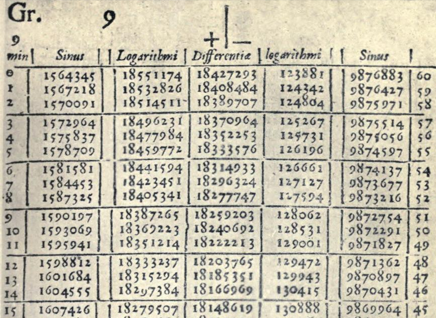
\includegraphics[scale=.3]{./napier.png}
  \end{figure}
\end{frame}

\begin{frame}
  \frametitle{Logarithm Charts I}
  A logarithm chart has a left-hand column for $y$ and a right-hand
  column for $x$ such that $a^{x}=y$. Here is an example, taking
  $a=10$.
\begin{tabular}{|r|r|r|r|}\hline
1  & 0.00000 & $\vdots$ & $\vdots$ \\ \hline
2  & 0.30103 & 432      & 2.6355   \\ \hline
3  & 0.47712 & $\vdots$ & $\vdots$ \\ \hline
4  & 0.60206 & 703      & 2.8470   \\ \hline
5  & 0.69897 & $\vdots$ & $\vdots$ \\ \hline
6  & 0.77815 & 303696   & 5.4825   \\ \hline
7  & 0.84510 & $\vdots$ & $\vdots$ \\ \hline
8  & 0.90309 &          &          \\ \hline
9  & 0.95424 &          &          \\ \hline
10 & 1.00000 &          & \\ \hline
\end{tabular}
\end{frame}

\begin{frame}
  \frametitle{Logarithm Charts II}
  Imagine you have no calculator and you need to multiply
  $432\cdot{}703$. It would take a while to do by hand! Alternatively,
  you could use a logarithm chart, look up the logarithms for $432$
  and $703$, add them (as opposed to multiplying!), and then look up
  which number corresponds to the resulting logarithm.
  \begin{equation}
    \label{eq:imohbise}
    432\cdot{}703=10^{2.6355}\cdot{}10^{2.8470}=\notag
  \end{equation}
  \begin{equation}
    \label{eq:maighaiw}
    10^{2.6355+2.8470}=10^{5.4825}=303696
  \end{equation}
\end{frame}

\begin{frame}
  \frametitle{Properties of the Logarithm}
  \begin{itemize}
  \item The domain of $\log_{a}$ is all the positive real numbers.
  \item The range of $\log_{a}$ is the whole number line $\mathbb{R}$.
  \item The logarithm of $y=1$ is always $0$. \emph{Reason:}
    $a^{0}=1$.
  \item The logarithm of the base $y=a$ is always $1$. \emph{Reason:}
    $a^{1}=a$.
  \item The logarithm of $y=a^{x}$ is always $x$. \emph{Reason:}
    $a^{x}=a^{x}$.
  \item $a$ to the power of $\log_{a}y$ is $y$. \emph{Reason:} that's
    precisely the definition of the logarithmic function.
  \end{itemize}
\end{frame}

\begin{frame}
  \frametitle{Laws of Logarithms}
Here are some laws, all of which make sense in terms of what we have
learned so far. 
\begin{equation}
  \label{eq:xeechahk}
\log_{a}(AB)=\log_{a}A+\log_{a}B
\end{equation}
\begin{equation}
  \label{eq:lahmophu}
\log_{a}\left(\frac{A}{B}\right)=\log_{a}A-\log_{a}B
\end{equation}
\begin{equation}
  \label{eq:ifohvoom}
\log_{a}(A^{C})=C\cdot \log_{a}A
\end{equation}
$A$ and $B$ must be positive real numbers for these laws to be
generally valid. For example, $\log((-2)\cdot(-2))\neq\log(-2)+\log(-2)$.
\end{frame}

\begin{frame}
  \frametitle{What Not to Do}
Make sure that you \textbf{do not} apply the laws of logarithms the
wrong way around!
\begin{equation}
  \label{eq:iotaegei}
\mbox{log}_{a}(x+y)\alert{\neq}\mbox{log}_{a}x+\mbox{log}_{a}y
\end{equation}
\begin{equation}
  \label{eq:phaamaje}
\frac{\mbox{log}_{a}x}{\mbox{log}_{a}y}\alert{\neq}\mbox{log}_{a}x-\mbox{log}_{a}y
\end{equation}
\begin{equation}
  \label{eq:luhaelae}
(\mbox{log}_{a}x)^{3}\alert{\neq}{}3\mbox{log}_{a}x
\end{equation}
Notation: sometimes we write $\ln{}x$ instead of $\log_{e}(x)$.
$\log_{e}$ is also called the \alert{natural logarithm}.
\end{frame}

\begin{frame}
  \frametitle{Change of Base Law}
Suppose you know what $\mbox{log}_{a}x$ is but you want to know what
$\mbox{log}_{b}x$ is. Consider the following equivalent equations:
\begin{equation}
  \label{eq:oovaeyah}
  y=\log_{b}x
\end{equation}
\begin{equation}
  \label{eq:bahsheep}
  b^{y}=x
\end{equation}
\begin{equation}
  \label{eq:mahteizo}
  \mbox{log}_{a}(b^{y})=\mbox{log}_{a}x
\end{equation}
\begin{equation}
  \label{eq:goonaera}
  y\mbox{log}_{a}b=\mbox{log}_{a}x
\end{equation}
\begin{equation}
  \label{eq:pieghoox}
  y=\frac{\mbox{log}_{a}x}{\mbox{log}_{a}b}
\end{equation}
This proves the Change of Base Formula:
\begin{equation}
\label{eq:seengahj}
  \mbox{log}_{b}x=\frac{\mbox{log}_{a}x}{\mbox{log}_{a}b}
\end{equation}
\end{frame}

\begin{frame}
  \frametitle{Exercises}
{\ubung} Express 
\begin{equation}
\label{eq:theethee}
3\ln{}x+\frac{1}{2}\ln{}(x+1) 
\end{equation}
as a single logarithm. 

{\ubung} Analyze the expression 
\begin{equation}
\label{eq:eeghogaf}
\mbox{log}_{12}\left(\frac{x^{3}}{y^{\frac{1}{2}}}\right)
\end{equation}

{\ubung} What is 
\begin{equation}
\label{eq:ouquaiko}
\ln{}\ln{}e^{e^{\mbox{\tiny ln}e^{x}}}
\end{equation}
\end{frame}

\begin{frame}
  \frametitle{Exercises}
{\ubung} Show that 
\begin{equation}
\label{eq:nuocaeph}
-\ln{}\left(x-\sqrt{x^{2}-1}\right)=\ln{}\left(x+\sqrt{x^{2}-1}\right)
\end{equation}

{\ubung} Use the Change of Base Formula and the calculator to evaluate
$\mbox{log}_{7}24$ and $\mbox{log}_{3}59049$.
\end{frame}

\begin{frame}
  \frametitle{Exercises}
{\ubung} Rewrite the expression as a single logarithm,
\begin{equation}
  \label{eq:zahshaum}
\ln(a+b)+\ln(a-b)-2\ln{}c
\end{equation}

{\ubung} Use the change of base formula and the natural logarithm to
evaluate: $\log_{4}125$

{\ubung} Analyze the expression so there is no longer a logarithm of a
product, quotient, root, or power: 
\begin{equation}
  \label{eq:ooreyonu}
  \log\left(\frac{a^{2}}{b^{4}\sqrt{c}}\right)
\end{equation}
\end{frame}

\begin{frame}
  \frametitle{End of Lesson}
Next Lesson: Log/Expo Equations
\end{frame}

\end{document}
